%------------------------------------------------
\section{Desenho e implementação}
%------------------------------------------------

%%%%%%%%%%%%%%%%%%%%%%%%%%%%%%%%%%%%%%%%%%%%%%%%%%%%%%%%%%%
%%%%%%%%%%%%%%%%%%%%%%%%%%%%%%%%%%%%%%%%%%%%%%%%%%%%%%%%%%%
\subsection{Projeto do \textit{hardware}}

\begin{frame}
\frametitle{Desenho e implementação}

Projeto do \textit{Hardware}

\begin{figure}[th]
	\centering
	\captionsetup{width=0.65\textwidth,font=footnotesize,textfont=bf}
	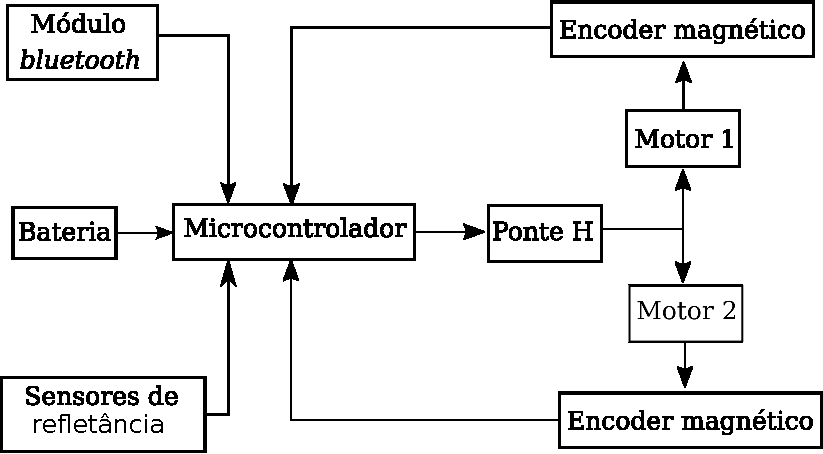
\includegraphics[width=0.65\textwidth,keepaspectratio]{Figuras/DiagramaHW.pdf}
	\caption{Diagrama de funcionamento do \textit{hardware} do veículo.\label{fig:diagEl}}
\end{figure}

\end{frame}

%% ----------------------------------------------------

\begin{frame}
\frametitle{Sensores e condicionamento de sinais}

\begin{figure}[th]
	\centering
	\captionsetup{width=0.65\textwidth,font=footnotesize,textfont=bf}
	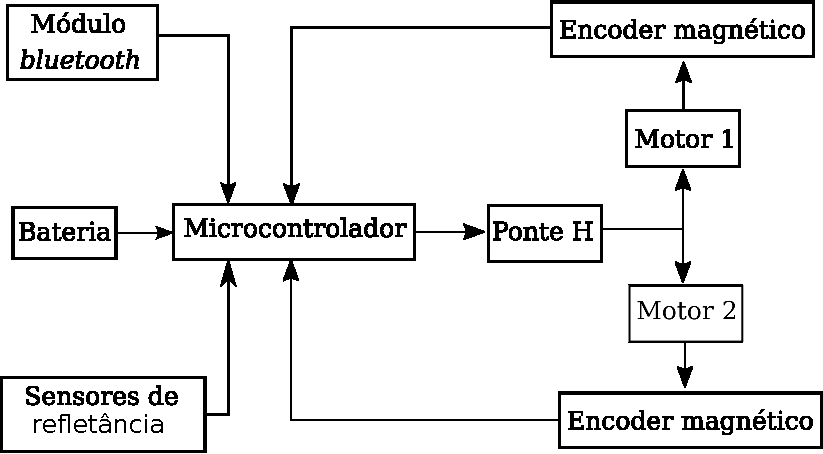
\includegraphics[width=0.65\textwidth,keepaspectratio]{Figuras/DiagramaHW.pdf}
	\caption{Diagrama de funcionamento do \textit{hardware} do veículo.\label{fig:diagEl}}
\end{figure}


\end{frame}

%% To not change the number page of this slide
\begin{frame}[noframenumbering]
\frametitle{Sensores e condicionamento de sinais}



    \transglitter
    \frametitle{Test}
        \begin{itemize}
            \item One
            \item Two
            \item Three
        \end{itemize}
\end{frame}

%% ------------------------------------------------------

\begin{frame}
\frametitle{Sensor de refletância QRE1113}

\begin{figure}[th]
	\centering
	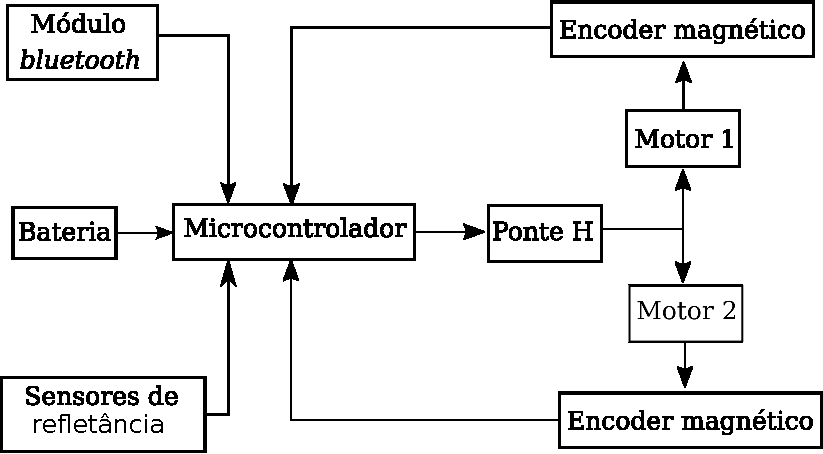
\includegraphics[width=0.65\textwidth,keepaspectratio]{Figuras/DiagramaHW.pdf}
	\caption{Diagrama de funcionamento do \textit{hardware} do veículo.\label{fig:diagEl}}
\end{figure}
\end{frame}

%% ------------------------------------------------------

\begin{frame}
\frametitle{\textit{Driver} de acionamento TB6612FNG}

\begin{figure}[th]
	\centering
	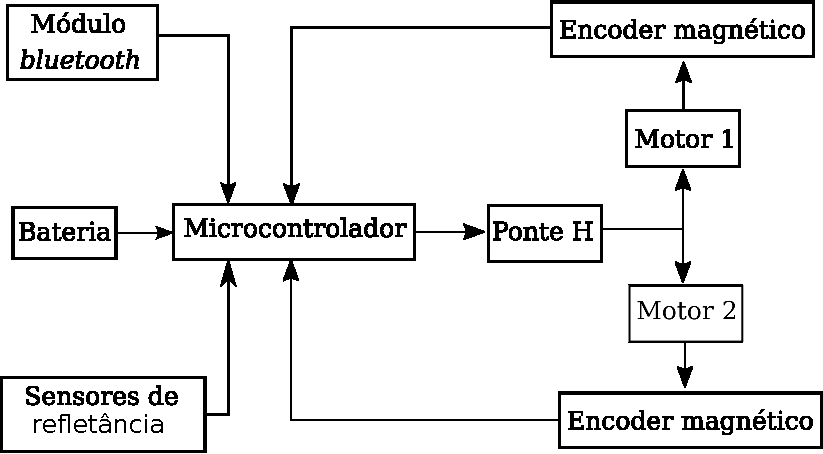
\includegraphics[width=0.65\textwidth,keepaspectratio]{Figuras/DiagramaHW.pdf}
	\caption{Diagrama de funcionamento do \textit{hardware} do veículo.\label{fig:diagEl}}
\end{figure}
\end{frame}

%% ------------------------------------------------------



%%%%%%%%%%%%%%%%%%%%%%%%%%%%%%%%%%%%%%%%%%%%%%%%%%%%%%%%%%%
%%%%%%%%%%%%%%%%%%%%%%%%%%%%%%%%%%%%%%%%%%%%%%%%%%%%%%%%%%%
\subsection{Projeto do controlador de SED}

\begin{frame}
\frametitle{Projeto do controlador de SED}
\begin{columns}
	\column{0.4\linewidth}
		\begin{itemize}
		\item Modelado pelos \textit{softwares} Supremica e Deslab
		\item Autômato de Moore
		\item Variáveis mapeadas:
			\begin{itemize}
			\item B1 (botão);
			\item AcharDir;
			\item PerdeDir;
			\item AchaEsq;
			\item PerdeEsq.
			\end{itemize}
		\end{itemize}
	\column{0.7\linewidth}
		\begin{figure}[th]
		\centering
		\captionsetup{width=\textwidth,font=footnotesize,textfont=bf}
		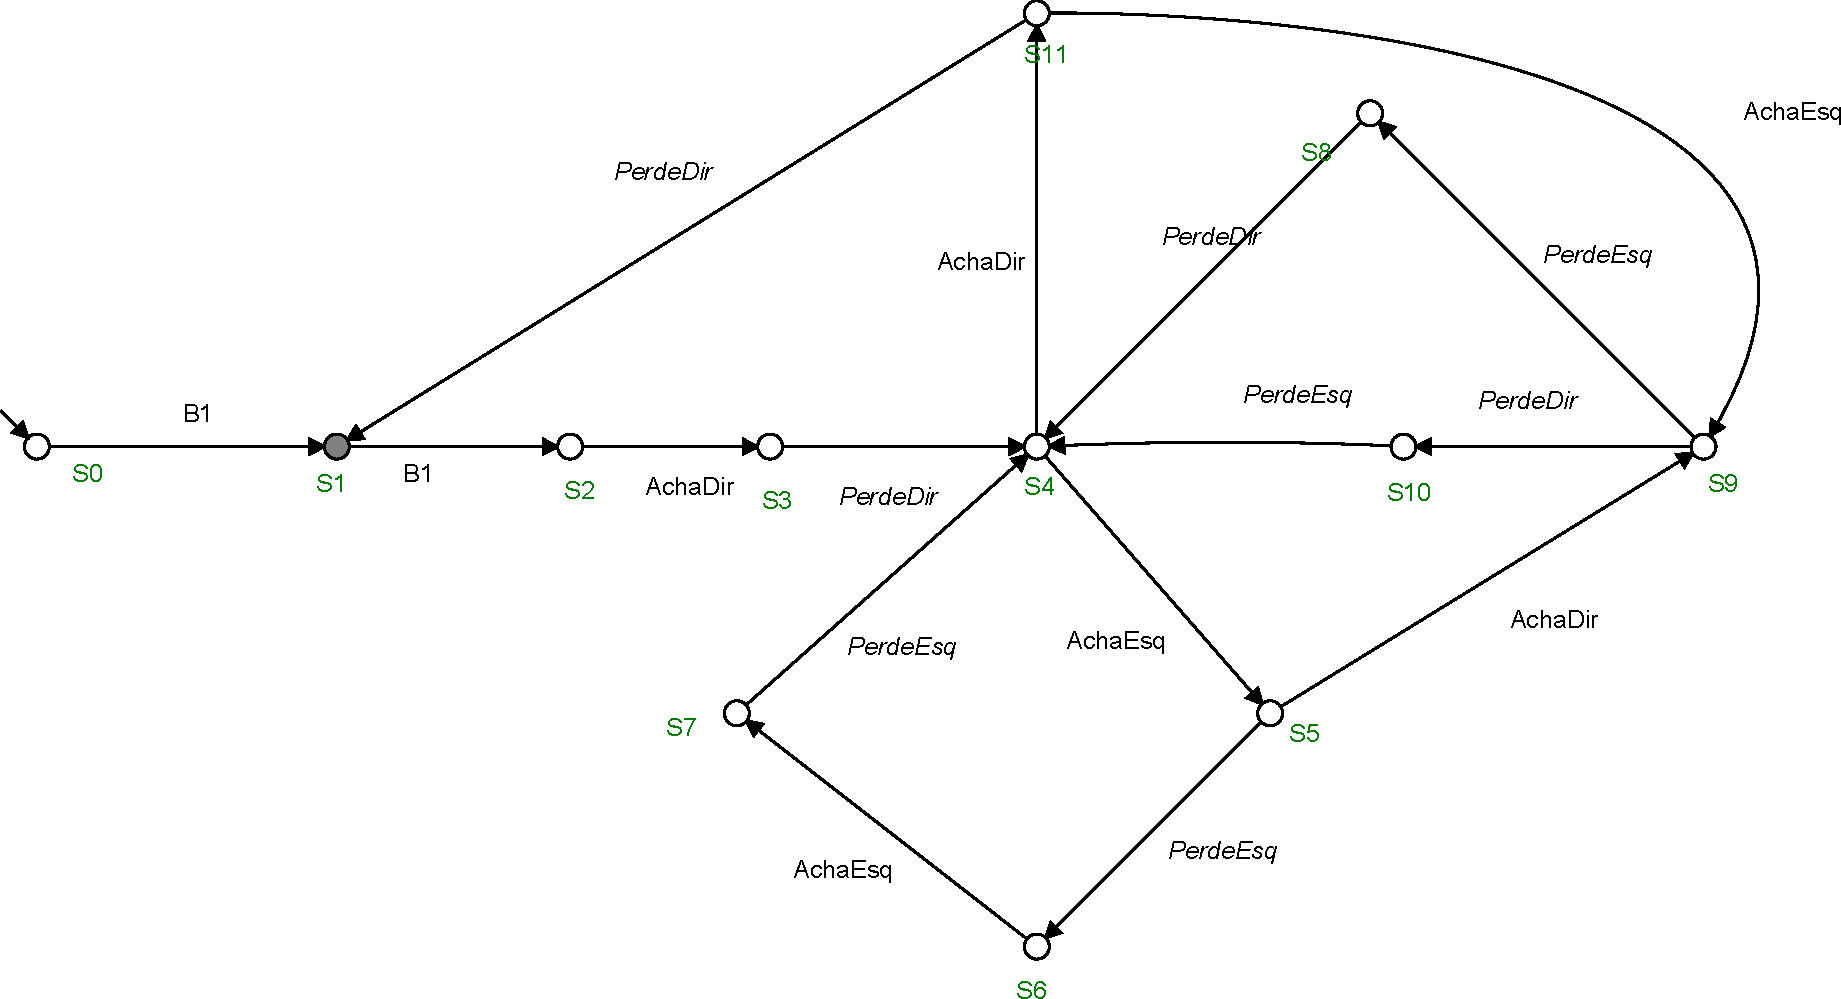
\includegraphics[width=\textwidth,keepaspectratio]{Figuras/SED.pdf}
		\caption{Controlador de SED}				
		\end{figure}
\end{columns}

\end{frame}

%%%%%%%%%%%%%%%%%%%%%%%%%%%%%%%%%%%%%%%%%%%%%%%%%%%%%%%%%%%
%%%%%%%%%%%%%%%%%%%%%%%%%%%%%%%%%%%%%%%%%%%%%%%%%%%%%%%%%%%
\subsection{Projeto do sistema de mapeamento}

\begin{frame}
\frametitle{Projeto do sistema de mapeamento}
\begin{columns}
	\column{0.4\linewidth}
		\begin{itemize}
		\item Armazenamento na memória \textit{flash}
		\item Contém as seguintes informações:
			\begin{itemize}
			\item Quantidade de marcações;
			\item Início e fim de marcação da direita;
			\item Início e fim de marcação da esquerda;
			\end{itemize}
		\end{itemize}
	\column{0.7\linewidth}
		\begin{figure}[th]
		\centering
		\captionsetup{width=\textwidth,font=footnotesize,textfont=bf}
		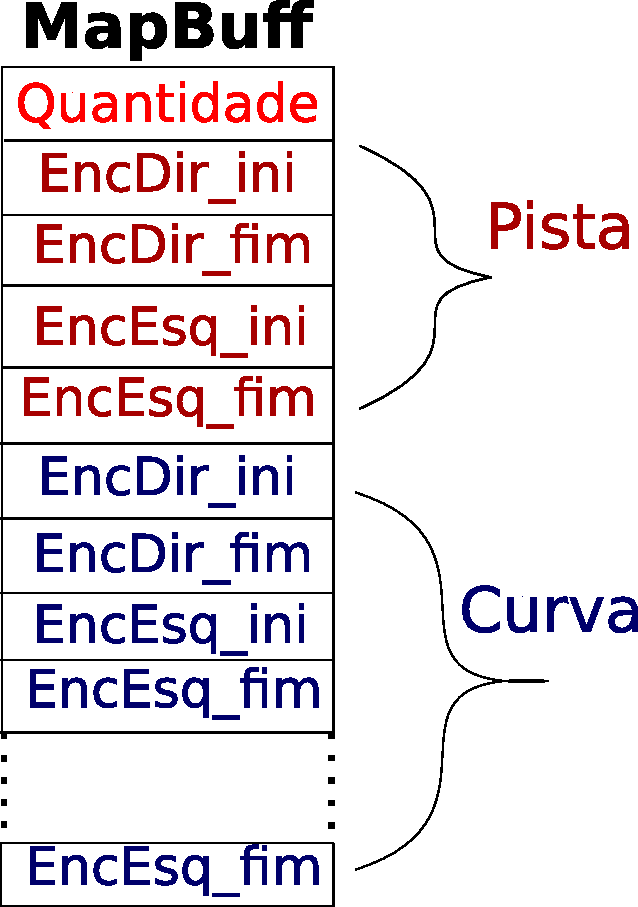
\includegraphics[width=0.6\linewidth,keepaspectratio]{Figuras/VetorMap.pdf}
		\caption{Vetor de armazenamento na \textit{flash}}				
		\end{figure}
\end{columns}

\end{frame}

%%%%%%%%%%%%%%%%%%%%%%%%%%%%%%%%%%%%%%%%%%%%%%%%%%%%%%%%%%%
%%%%%%%%%%%%%%%%%%%%%%%%%%%%%%%%%%%%%%%%%%%%%%%%%%%%%%%%%%%
\subsection{Função de transferência do veículo}

\begin{frame}
\frametitle{Função de Transferência do veículo}
\textbf{Aquisição dos valores da planta}
\begin{columns}
	\column{0.4\linewidth}
		\begin{itemize}
		\item Obtenção da posição
		\item Mesmo PWM para os motores
		\item Motores em sentidos opostos
		\item Informações enviadas via \textit{bluetooth}
		\item É esperado um gráfico próximo a uma rampa
		\end{itemize}
	\column{0.7\linewidth}
		\begin{figure}[th]
		\centering
		\captionsetup{width=\textwidth,font=footnotesize,textfont=bf}
		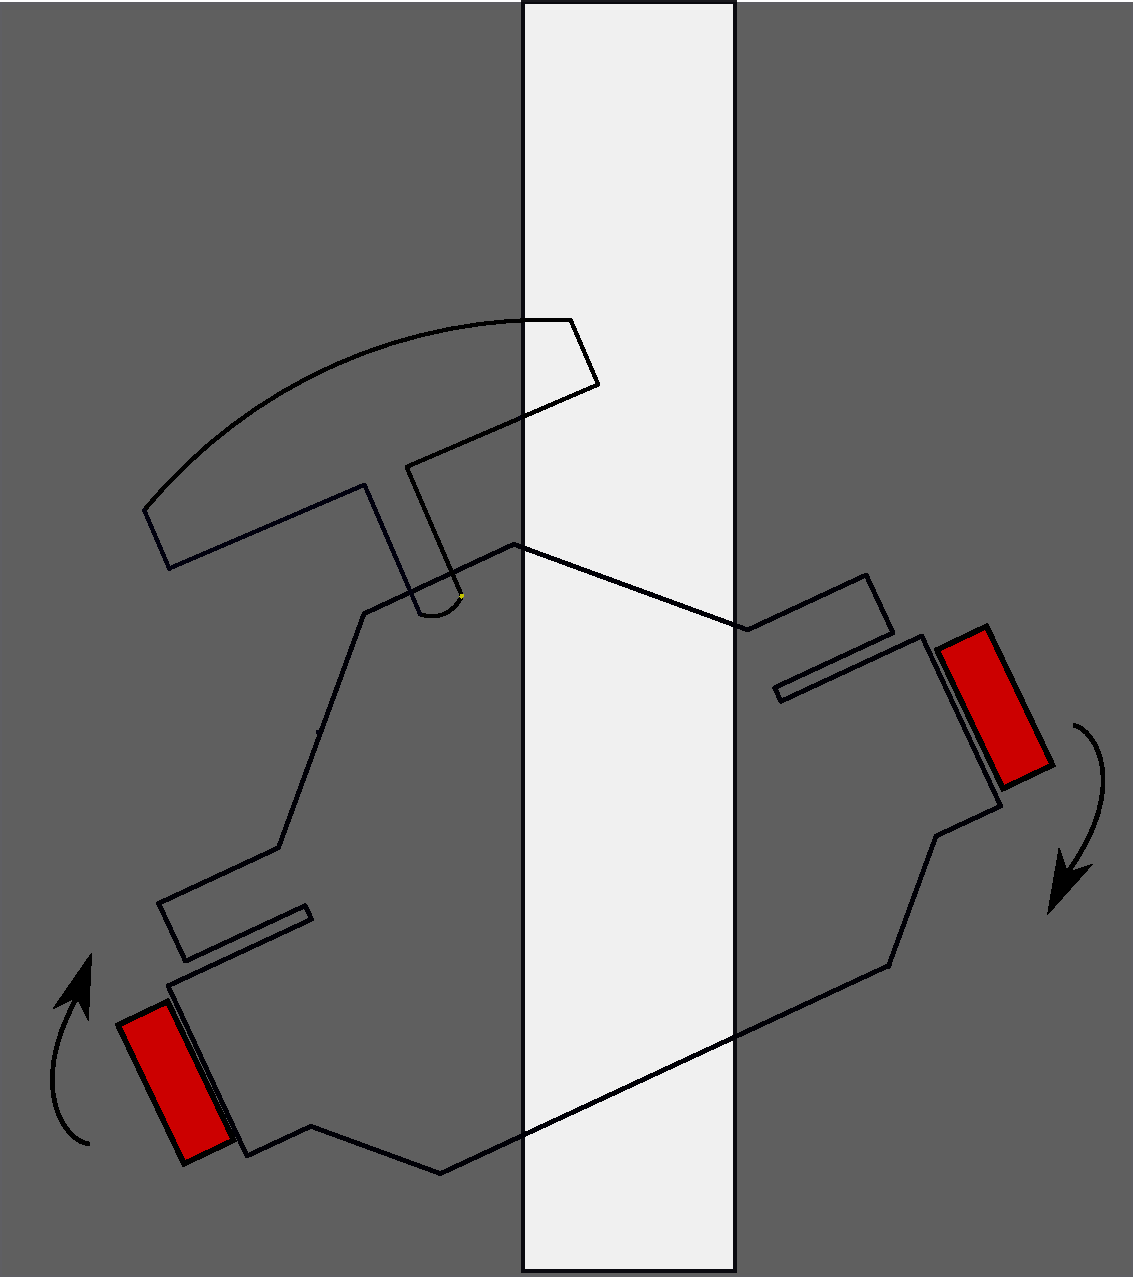
\includegraphics[width=0.6\linewidth,keepaspectratio]{Figuras/FT.pdf}
		\caption{Aquisição dos valores de posição do robô}				
		\end{figure}
\end{columns}
\end{frame}


\begin{frame}
\frametitle{Função de Transferência do veículo}
\textbf{Modelo da função de transferência}\\
	Para encontrar a velocidade, deriva-se a posição
	
\begin{columns}
	\column{0.5\linewidth}

	\begin{figure}[th]
	\centering
	\captionsetup{width=\textwidth,font=footnotesize,textfont=bf}
	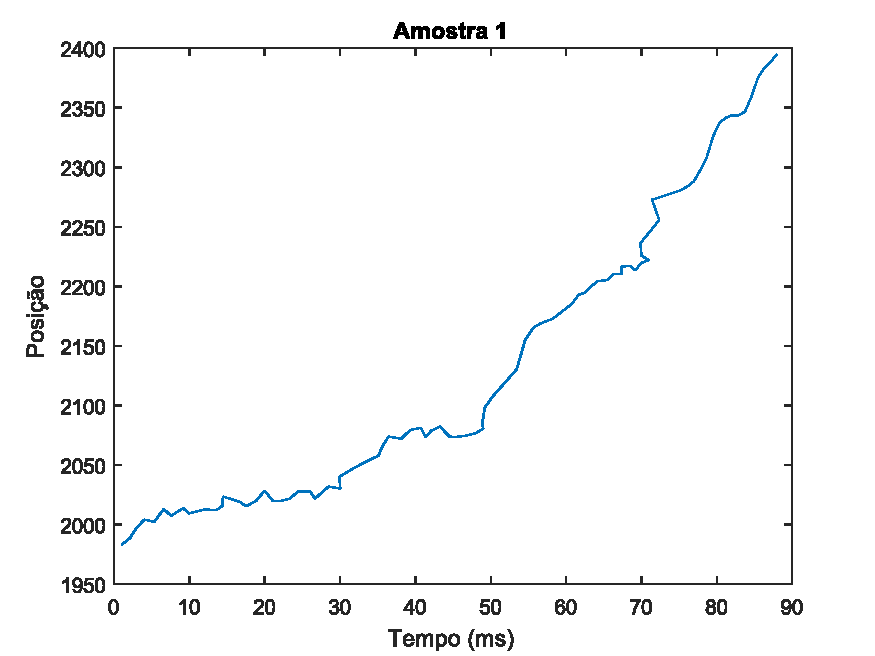
\includegraphics[width=\linewidth,keepaspectratio]{Figuras/Posicao3v2.pdf}
	\caption{Gráfico da posição obtida}				
	\end{figure}
 	
	%\pause 	
 	\column{0.5\linewidth}
	\begin{figure}[th]
	\centering
	\captionsetup{width=\textwidth,font=footnotesize,textfont=bf}
	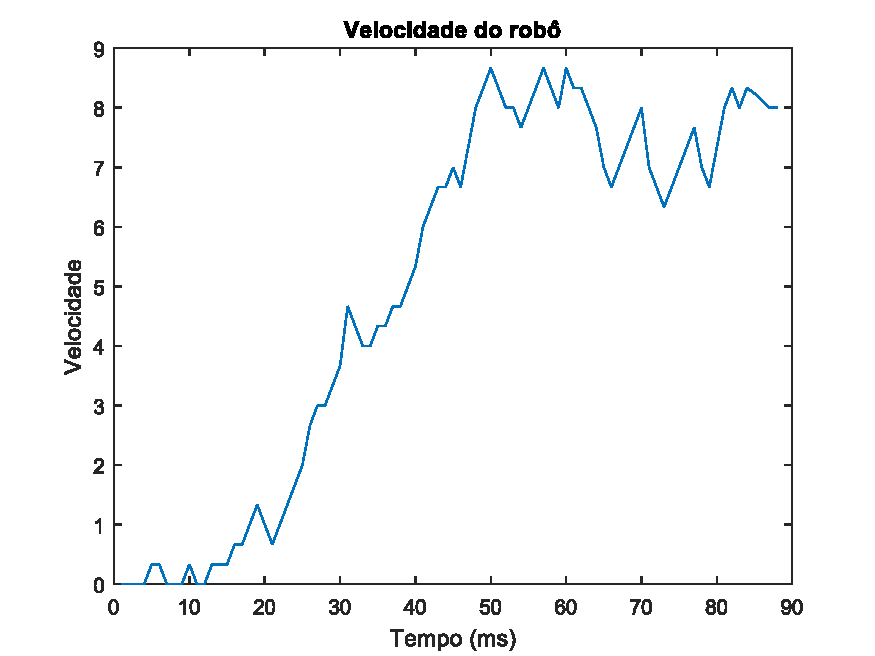
\includegraphics[width=\linewidth,keepaspectratio]{Figuras/Derivadav2.pdf}
	\caption{Gráfico da velocidade}				
	\end{figure}
\end{columns}
\end{frame}



\begin{frame}
\frametitle{Função de Transferência do veículo}
\textbf{Modelo da função de transferência}\\
Com o Matlab, verificou-se uma função que mais se aproxima da desejada
	
\begin{columns}
 		
 	\column{0.45\linewidth}
 	\vspace{-0.5cm}
 	\begin{itemize}
 	\item $P2ZU = 0,0054915(\frac{1-0,011087s}{1+0,014889s+0,000238s^2})$
 	\item A função contém 3 polos e 1 zero
 	\end{itemize}
 	
 	\column{0.55\linewidth}

	\begin{figure}[th]
	\centering
	\captionsetup{width=0.9\textwidth,font=footnotesize,textfont=bf}
	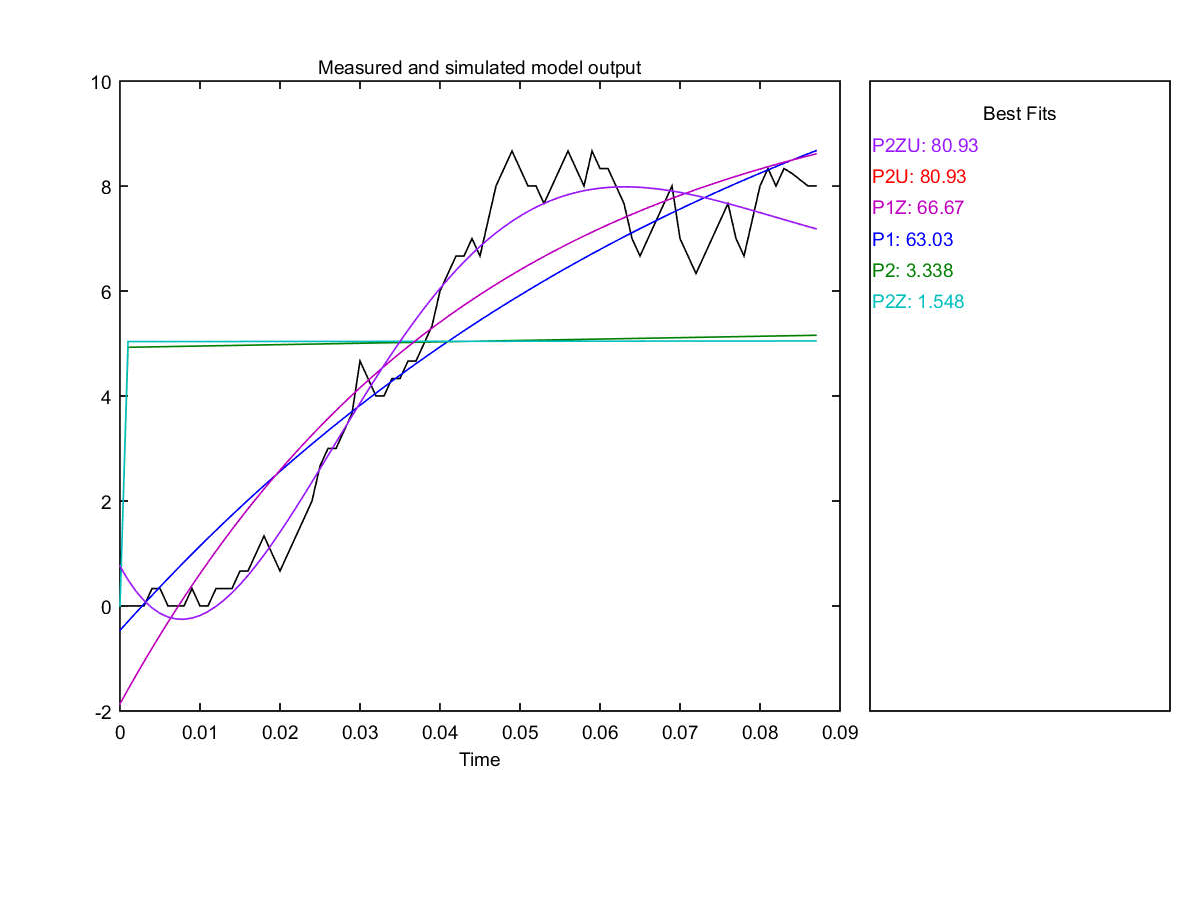
\includegraphics[width=\linewidth,keepaspectratio]{Figuras/Comparativo.pdf}
	\caption{Comparativo feito pelo System Identification}				
	\end{figure}
	
\end{columns}
\end{frame}

\begin{frame}
\frametitle{Função de Transferência do veículo}
\textbf{Modelo da função de transferência}\\
	
\begin{columns}

	\column{0.5\linewidth}
 	\begin{itemize}
 	\item A função encontrada é relacionada à velocidade
 	\item Para a original, é necessário integrá-la e multiplicá-la pelo ganho
 	\item $FT: 1223(\frac{P2Z2}{s})$
	\end{itemize} 		

 	\column{0.5\linewidth}
	\begin{figure}[th]
	\centering
	\captionsetup{width=0.85\textwidth,font=footnotesize,textfont=bf}
	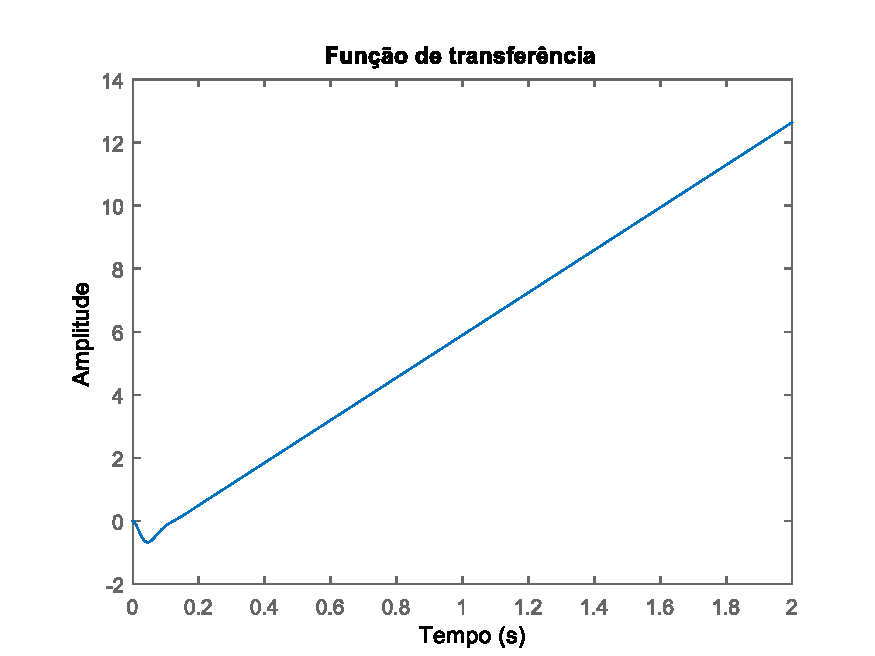
\includegraphics[width=\linewidth,keepaspectratio]{Figuras/planta2v2.pdf}
	\caption{Função de transferência encontrada}				
	\end{figure}
	
\end{columns}
\end{frame}

%%%%%%%%%%%%%%%%%%%%%%%%%%%%%%%%%%%%%%%%%%%%%%%%%%%%%%%%%%%
%%%%%%%%%%%%%%%%%%%%%%%%%%%%%%%%%%%%%%%%%%%%%%%%%%%%%%%%%%%
\subsection{Projeto do controlador de tempo contínuo}


\begin{frame}
\frametitle{Projeto do controlador de tempo contínuo}

\begin{itemize}
\item Controlador Proporcional-Derivativo (PD)
\item Variável controlada é a posição
\end{itemize}

\begin{equation}\label{eq:posicao}
posicao = \frac{\sum_{n=1}^{5} 1000(n-1)V_{n}}{\sum_{n=1}^{5} V_{n}}
\end{equation}

\begin{equation}\label{eq:posicao2}
posicao = \frac{0*V_{1} + 1000*V_{2} + 2000*V_{3} + 3000*V_{4} + 4000*V_{5} }{V_{1} + V_{2} + V_{3} + V_{4} + V_{5}}
\end{equation}

\end{frame}

%%% VER PARA TALVEZ COLOCAR O CODIGO DO PD CONTROLLER

%
%\begin{frame}
%\frametitle{Theorem}
%\begin{theorem}[Mass--energy equivalence]
%$E = mc^2$
%\end{theorem}
%\end{frame}


\begin{frame}[fragile] % Need to use the fragile option when verbatim is used in the slide
\frametitle{Verbatim}
\begin{example}[Theorem Slide Code]
\begin{verbatim}
\begin{frame}
\frametitle{Theorem}
\begin{theorem}[Mass--energy equivalence]
$E = mc^2$
\end{theorem}
\end{frame}\end{verbatim}
\end{example}
\end{frame}



%\begin{figure}[H]
%     \centering
%     \captionsetup{width=0.7\textwidth,font=footnotesize,textfont=bf}
%     \begin{subfigure}[b]{\textwidth}
% 	\centering
%         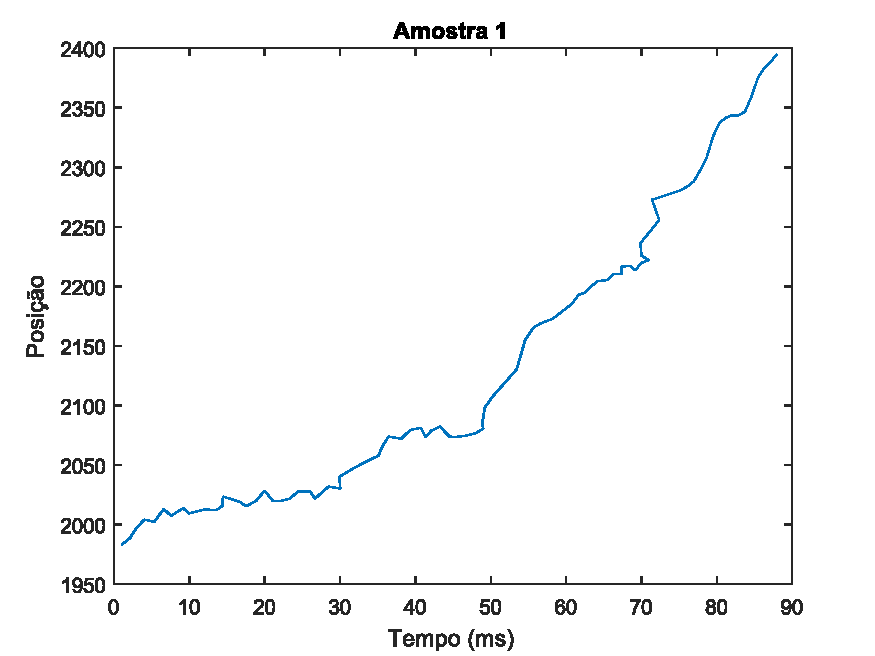
\includegraphics[width=0.6\textwidth,height=\textheight,keepaspectratio]{figuras/Posicao3v2.pdf}
%         \caption{\centering \label{fig:Posicaofinal}}
%     \end{subfigure}
%     
%     \begin{subfigure}[b]{\textwidth}
% 	\centering
%         \includegraphics[width=0.8\textwidth,height=0.3\textheight,keepaspectratio]{figuras/Posicaofinalv2.pdf}
%         \caption{\centering \label{fig:Posicao1}}
%     \end{subfigure}
%
%     \caption{Gráficos da posição em função do tempo (ms), com frequência de 16 KHz e \textit{duty cycle} de 30\%: (a) Amostra 1; (b) Amostra 2 \label{fig:posicoes}}
%     \vspace{-0.3cm}
%     \caption*{Fonte: Autoria própria}
% \end{figure}


%------------------------------------------------

